\chapter{Level2 processor and I/O data}

\begin{figure}[t]
\centering
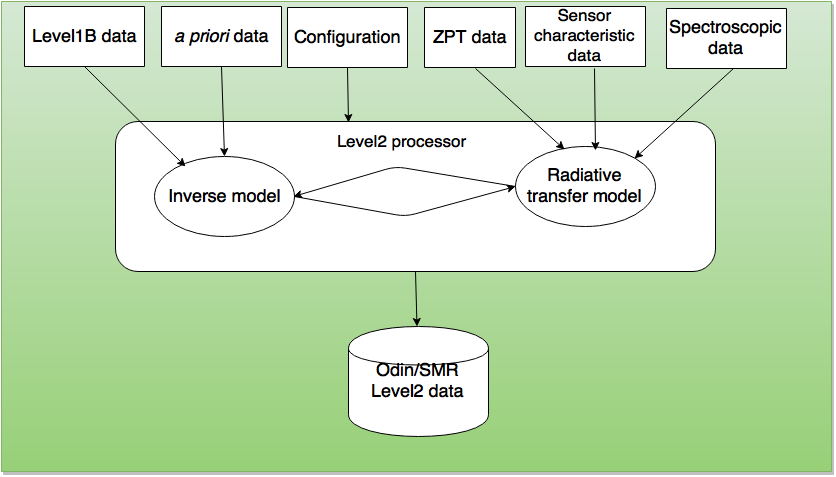
\includegraphics[width=14cm]{smr-level2-processor.png}
\caption{Schematic of the I/O data used and generated by the \smr\ Level2 processor.}
\label{fig:level2}
\end{figure}

\section{Level2 processor overview}

The \smr\ Level2 processor is designed to process
measurements from a scan of \smr\ in order to
retrieve profiles of atmospheric species.    
The Level2 processor is an optimal estimation method (OEM)
implementation, which combines measurement
information with Ancillary/Auxiliary data
and applies a forward model, and an iterative
scheme is used to find a best solution.   
The details of the algorithms within the
\smr\ Level2 processor is described in \smr\ Level2 ATBD.

\section{Level2 processor input data}

Figure~\ref{fig:level2} describes, on a high level, the input data used
by the Level2 processor and the generated output data.
\smr\ applies a number of different observation modes,
but the Level2 processor is identical for the various modes,
in terms of the high level workflow.

The Level2 processor obtains the input data through a hierarcical 
REST API, and the API is described in Sect.~\ref{sec:api}.
A high level description of the input data is described 
in the proceeding sections, and the detailed data formats
are described in Appendix~\ref{sec:dataformat}.


\subsection{Level1B data}
The most basic input data to the Level2 processor is the Level1B data,
i.e. geolocated and calibrated spectra from a scan of \smr.

\subsection{Climatological \textit{apriori} data}

Climatology data, covering all species of interest is required, as
the OEM implementation needs a starting estimate for each profile
to be retrieved. The climatology cover vertical, seasonal,
and latitudinal variations of each species and is based on data
from ?.

\subsection{ZPT data}
The Level2 processor requires external ZPT data (altitude, pressure, temperature) 
data. The ZPT data is extracted from the ERA-Interim dataset for the geolocation
of the scan. ERA-Interim is a global atmospheric reanalysis from 1979, and 
data is available throughout the Odin mission. 

\subsection{Sensor characteristic data}
The forward model simulation of the Level2 processor takes into account 
sensor characteristic data, i.e. the antenna angular response, 
sideband filtering, and frequency response of each spectrometer channel. 

\subsection{Spectroscopic data}
Spectroscopic data is basic input to the forward model of the Level2
processor.

\subsection{Configuration}
\smr\ applies a number of different observation modes,
and for each mode a different configuration is applied
of the Level2 processor...


\section{Level2 processor Output Data}
The output of the Level2 processor is retrieved
profiles of atmospheric species, error estimates,
and auxiliary data.
A high level description of the output data is described
in the proceeding sections, and the detailed data formats
are described in Appendix~\ref{sec:dataformat}.  

\subsection{Level2 data}
\subsection{Auxiliary data}

\section{API description}
\label{sec:api}

This section describes the API calls used to get data 
to the Level2 processing.
The data is accessed through a hierarcical REST API where deeper URIs return more
specific data.  All call URIs have a common root \url{rest_api/<version>}, which
has been omitted below for clarity.  All GET calls return JSON objects unless
otherwise noted. Key/value pairs are listed as name of the key
along with the type of the corresponding value within parantheses, followed
by a brief description of the contents.  
%See the sections on the different
%data sources for specifications on the structure of their respective JSON
%objects.


\subsection{API calls}

describe the various calls



